\begin{figure}
	\centering
	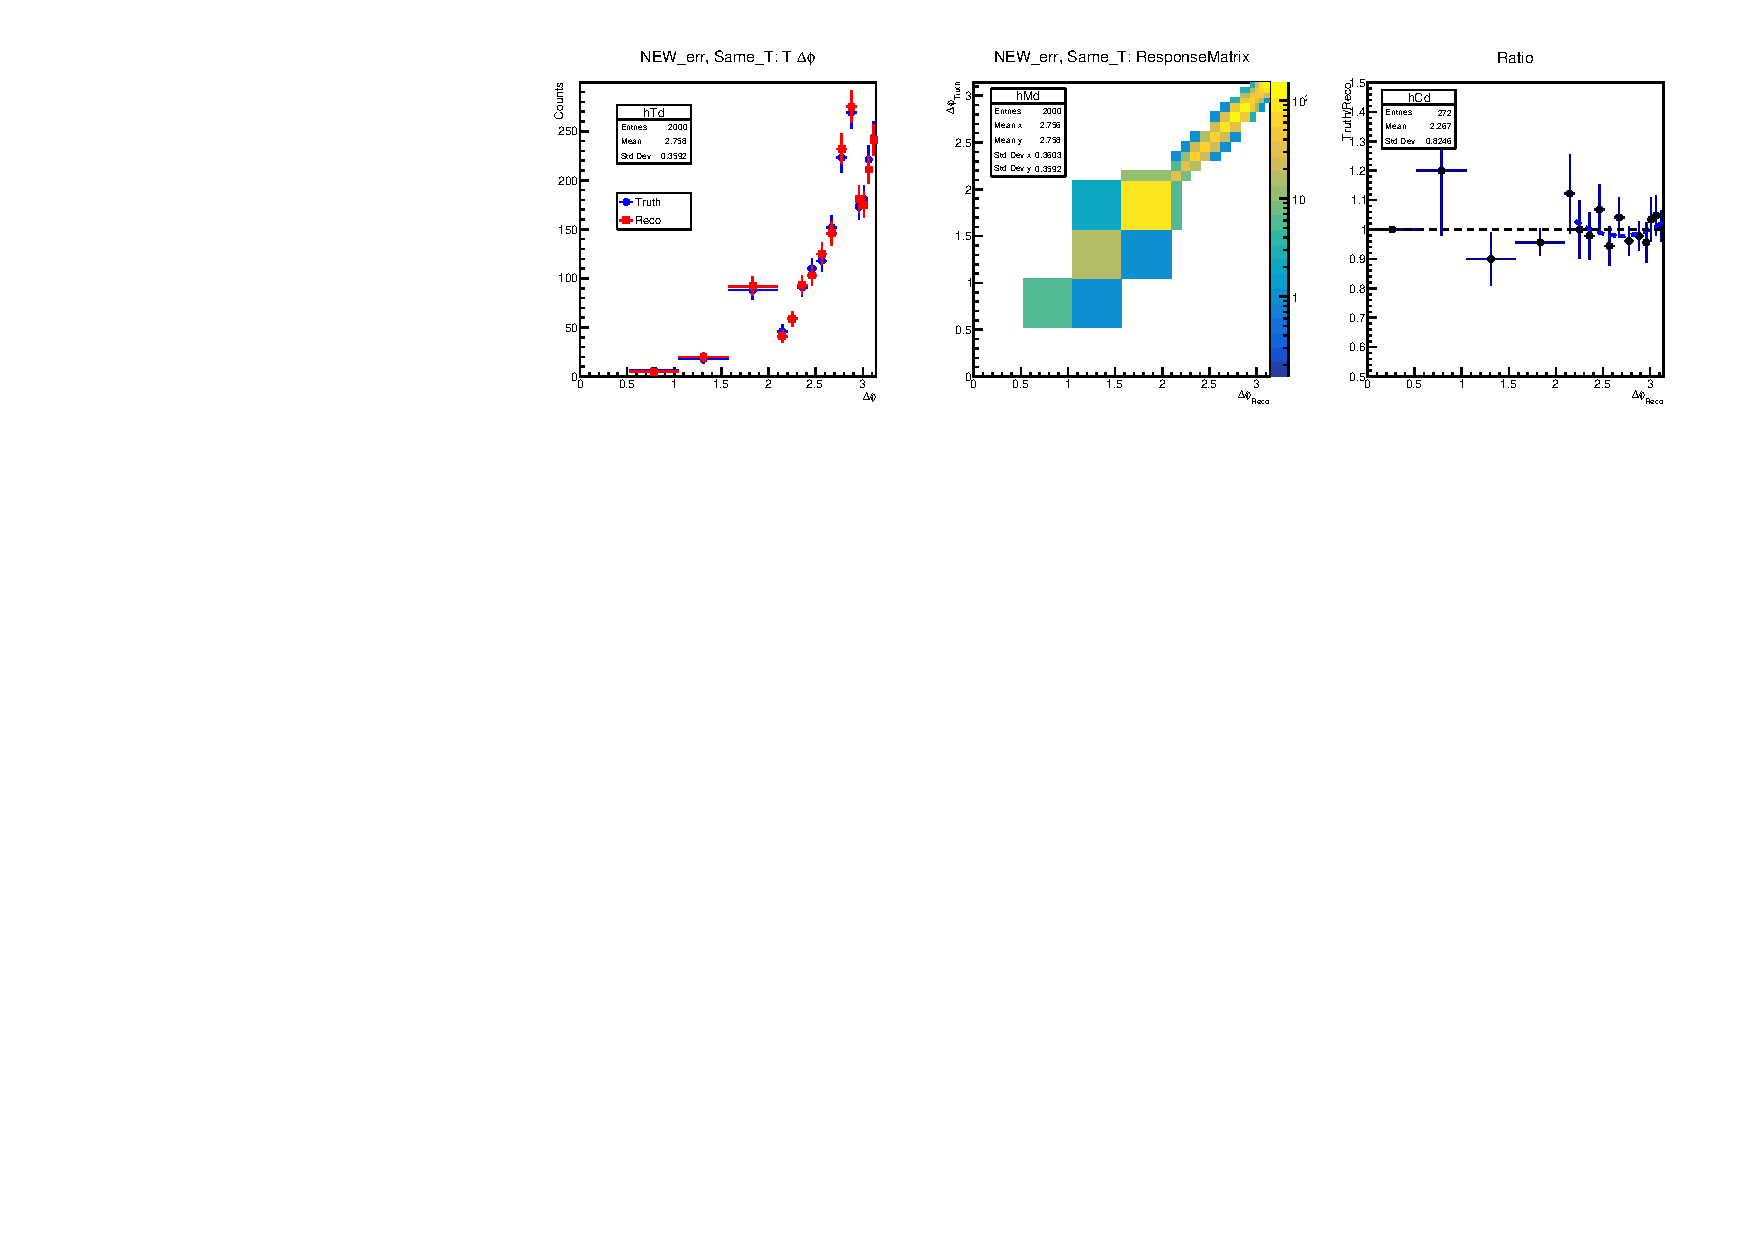
\includegraphics[width=1.0\textwidth]{figures/c.pdf} 
	\caption{ $\Delta\phi$ distributions for truth and reco (left). Response Matrix $M_{ij}$ (center). Correction factors with errors (right). }	
	\label{fig:plots}
\end{figure}

In Figure~\ref{fig:plots}, we have truth and reconstructed $\Delta\phi$ distributions on the left-most plot, the response matrix $M_{ij}$ where $\Delta\phi_{Reco}$ is along the x-axis, along the j-index, and $\Delta\phi_{Truth}$ is along the y-axis, along the i-index, and resulting correction factors with errors on the right-most. 

Define $T_{i}$ as the total number of entries in the $i^{th}$ bin of the Truth distribution (blue points on left plot), and $R_{i}$ as the total number of entries in the $i^{th}$ bin of the Reconstructed distribution (red points on left plot). 

In terms of the response matrix, $R_{j}$ is

\begin{eqnarray} \label{eq:rj}
R_j = \sum_{i}^{}M_{ij} = M_{jj} + \sum_{i\neq j}^{}M_{ij} 
\end{eqnarray}

The last part is just the diagonal element plus the off-diagonal vertical elements of the $i^{th}$ bin (on the x-axis).

Similarly, in terms of the response matrix, $T_{i}$ is

\begin{eqnarray} \label{eq:ti}
T_i = \sum_{j}^{}M_{ij} = M_{ii} + \sum_{j\neq i}^{}M_{ij} 
\end{eqnarray}

For some bin $i^{th}$ reconstructed bin,

\begin{eqnarray} \label{eq:leavearrive}
R_{i} = T_{i} - N_{Leaving} + N_{Arriving} = T_{i} - \sum_{k\neq i}^{}M_{ik} + \sum_{j\neq i}^{}M_{ji}
\end{eqnarray}

We can express the number leaving and number arriving in terms of off-diagonal row or column elements of $M_{ij}$, or in terms of  $T_{i}$, $R_{i}$, and diagonal elements of  $M_{ij}$.

\begin{eqnarray} \label{eq:leavearrivediagonal}
N_{Leaving} = T_{i} - M_{ii} \\
N_{Arriving} = R_{i} - M_{ii} 
\end{eqnarray}

Now, $T_{i}$ is taken as a constant. This means that reconstructed distribution can be different time to time, but the truth distribution stays the same. In the language of a toy MC, this is equivalent to generating one Truth distribution, and smearing it many different times, each time (or for each new "experiment") getting new results.

When $T_{i}$ is taken as constant, the bin migration of leaving and arriving is different. The distribution of $N_{Leaving}$ is binomial, while $N_{Arriving}$ is Poisson. If $T_{i}$ is fixed, there is only a certain number of entries that can leave, while the number that arrives depends on, and is a mix of the entries leaving neighboring bins. 

In a toy MC \footnote{A Toy MC with a randomly generated exponential was generated for the truth distribution 5000 times, with smearing from the ATLAS MC response matrix applied to the reconstructed distribution. The experiment was then repeated 10,000 times to get some good statistics on correction factors, their errors, bin migration, etc.}, for the case where the truth distribution was generated one time, but smearing applied to the reconstructed (case with "fixed" $T_{i}$), it is clear from Figure~\ref{fig:mig_same} that the migration where entries are leaving is narrower than where the arrive. In the same toy MC, when for every experiment a new truth distribution was used, it is evident that the migration to and from is the same.

\begin{figure}
	\centering
	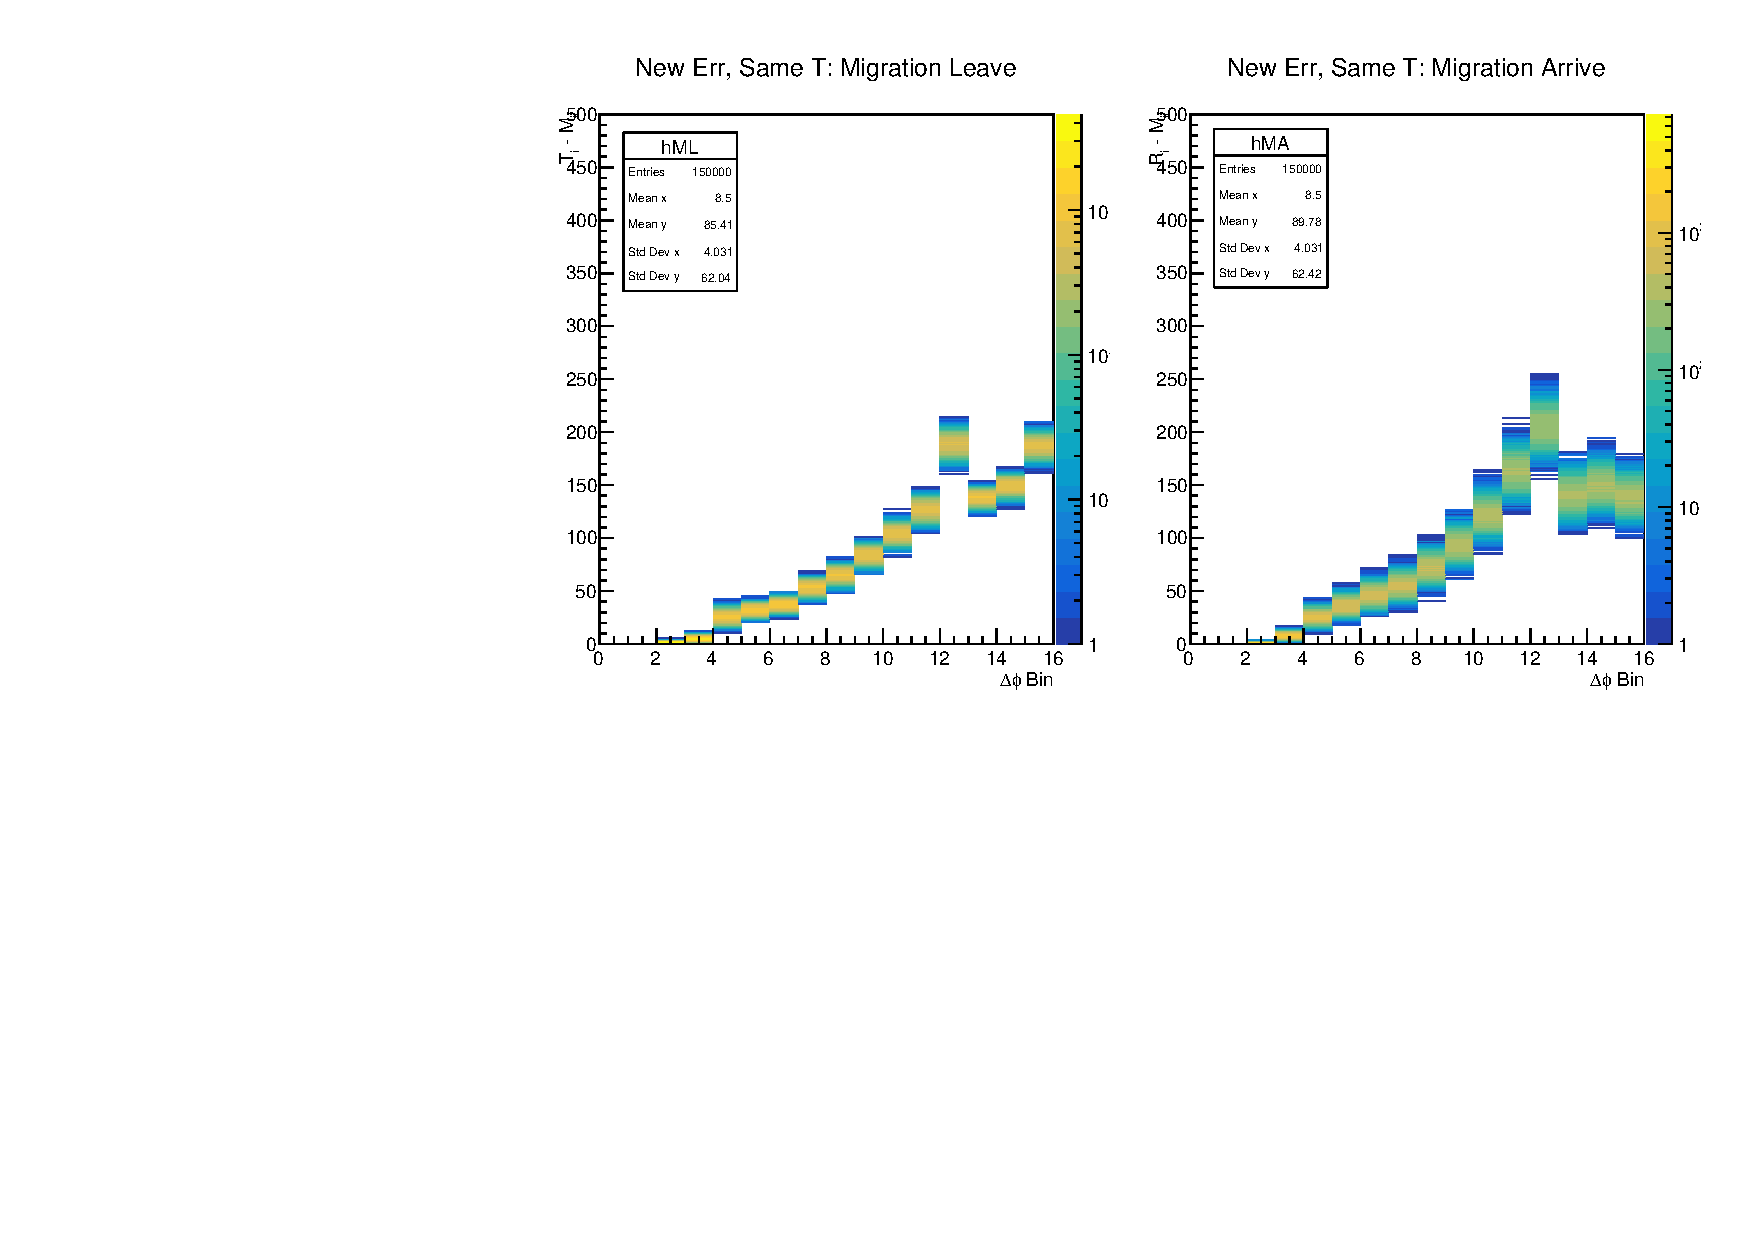
\includegraphics[width=1.0\textwidth]{figures/c3_same.pdf} 
	\caption{ For the case where for every experiment a the same generated truth distribution but differently smeared reconstructed distribution, histogram of migration between $\Delta\phi$ bins (x and y axes) for entries arriving (right) and entries leaving (left).Migration where entries leave has a binomial (narrower) distribution, while entries arriving is Poisson. }	
	\label{fig:mig_same}
\end{figure}

\begin{figure}
	\centering
	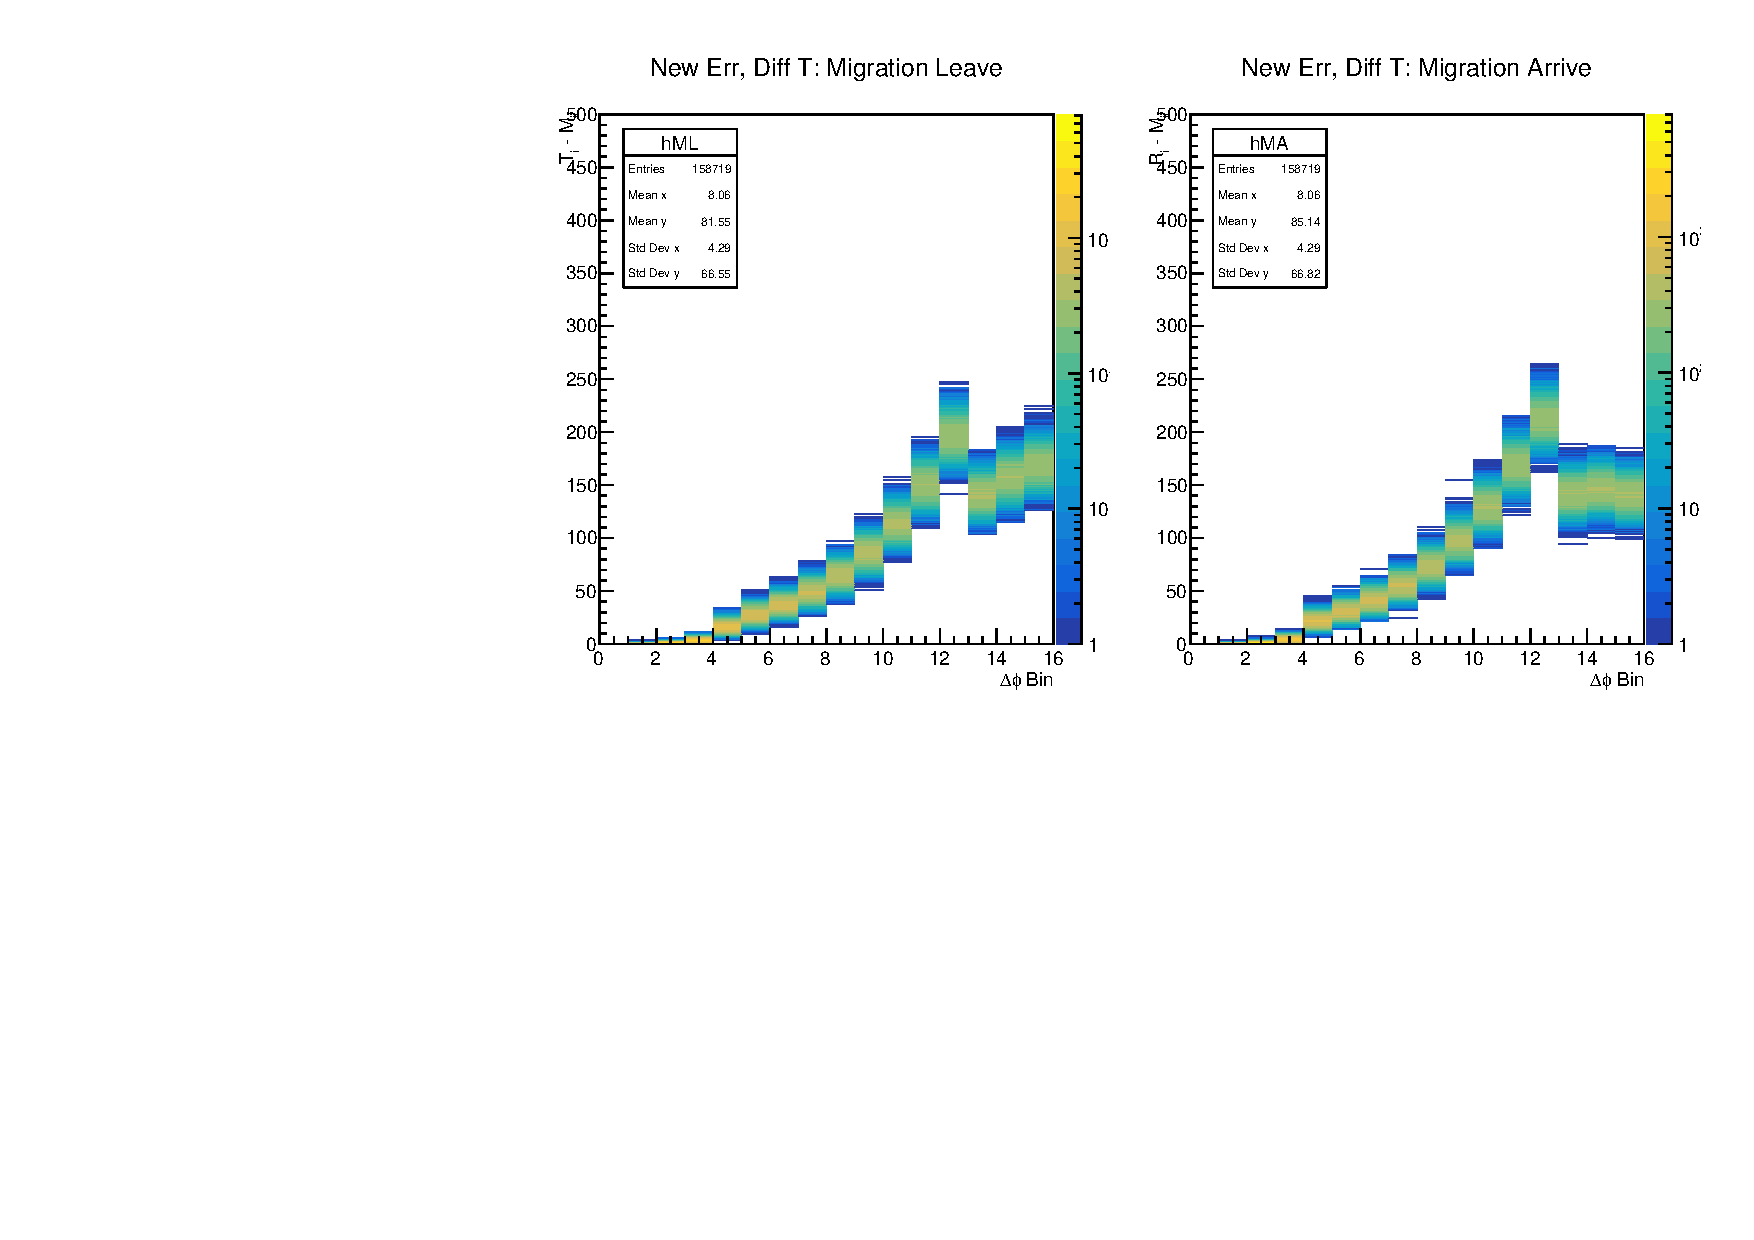
\includegraphics[width=1.0\textwidth]{figures/c3_diff.pdf} 
	\caption{ For the case where for every experiment a new truth distribution is generated and the reconstructed is smeared from that, histogram of migration between $\Delta\phi$ bins (x and y axes) for entries arriving (right) and entries leaving (left). Both migrations have Poisson distributions. }	
	\label{fig:mig_diff}
\end{figure}

Correction factors $C_{i}$, which relate $T_{i}$ and $R_{i}$ are

\begin{eqnarray} \label{eq:cfactors}
C_{i} = \frac{T_{i}}{R_{i}}
\end{eqnarray} 

and their respective errors $\sigma_{C_{i}}$ are

\begin{eqnarray} \label{eq:cfactorerrors}
\sigma_{C_{i}}^{2} = \frac{C_{i}^{2}}{R_{i}^{2}}\sigma_{R_{i}}^{2}
\end{eqnarray}	

Now since $T_{i}$ is constant, and the entries leaving a $T_{i}$ bin follow binomial statistics, while entries arriving are Poisson, we continue from Equation~\ref{eq:leavearrive}. The error in $R_{i}$ is 

\begin{eqnarray}
\sigma_{R_{i}}^{2} = \sigma_{N_{Leave}}^{2} + \sigma_{N_{Arrive}}^{2} \\ 
\sigma_{R_{i}}^{2} = T_{i}\frac{T_{i} - M_{ii}}{T_{i}}\big(1 - \frac{T_{i} - M_{ii}}{T_{i}}\big)+(R_{i}-M_{ii}) \\
\sigma_{R_{i}}^{2} = T_{i} + R_{i} - 2M_{ii} - \frac{(T_{i} - M_{ii})^{2}}{T_{i}}
\end{eqnarray}	

From this, plugging into Equation~\ref{eq:cfactorerrors}, the error on the correction factor is

\begin{eqnarray} \label{eq:cfactorerror}
\sigma_{C_{i}}^{2} = \frac{T_{i}^{2}}{R_{i}^{4}}\Big(T_{i} + R_{i} -2M_{ii} - \frac{(T_{i} - M_{ii})^{2}}{T_{i}}\Big) \\
\sigma_{C_{i}}^{2} = \frac{T_{i}^{2}}{R_{i}^{3}}\Big(1 - \frac{M_{ii}^{2}}{T_{i}R_{i}}\Big).
\end{eqnarray}	
